\definecolor{cfwone}{HTML}{eef5fa}
\definecolor{cfwtwo}{HTML}{daeaf5}
\definecolor{cfwthree}{HTML}{b2d2e9}
\definecolor{cfwfour}{HTML}{8abbde}

\newcommand{\fwone}[1]{\colbox{cfwone}{#1}\xspace}
\newcommand{\fwtwo}[1]{\colbox{cfwtwo}{#1}\xspace}
\newcommand{\fwthree}[1]{\colbox{cfwthree}{#1}\xspace}
\newcommand{\fwfour}[1]{\colbox{cfwfour}{#1}\xspace}

\newcommand{\fexp}[2]{\texttt{[{\color{darkgray}{#1:#2}}]}\xspace}
\newcommand{\fexptag}[1]{\fexp{TAG}{#1}}
\newcommand{\fexpfrom}[1]{\fexp{FROM}{#1}}
\newcommand{\fexpto}[1]{\fexp{TO}{#1}}
\newcommand{\fexptemp}[1]{\fexp{TEMP}{#1}}


\section{Counterfactual Explanations}

%Both counterfactual explanations and semi-counterfactual explanations.
%As defined in \cite{}

\subsection{Local explanations: Abnormality}





\begin{figure}[t]
\centering
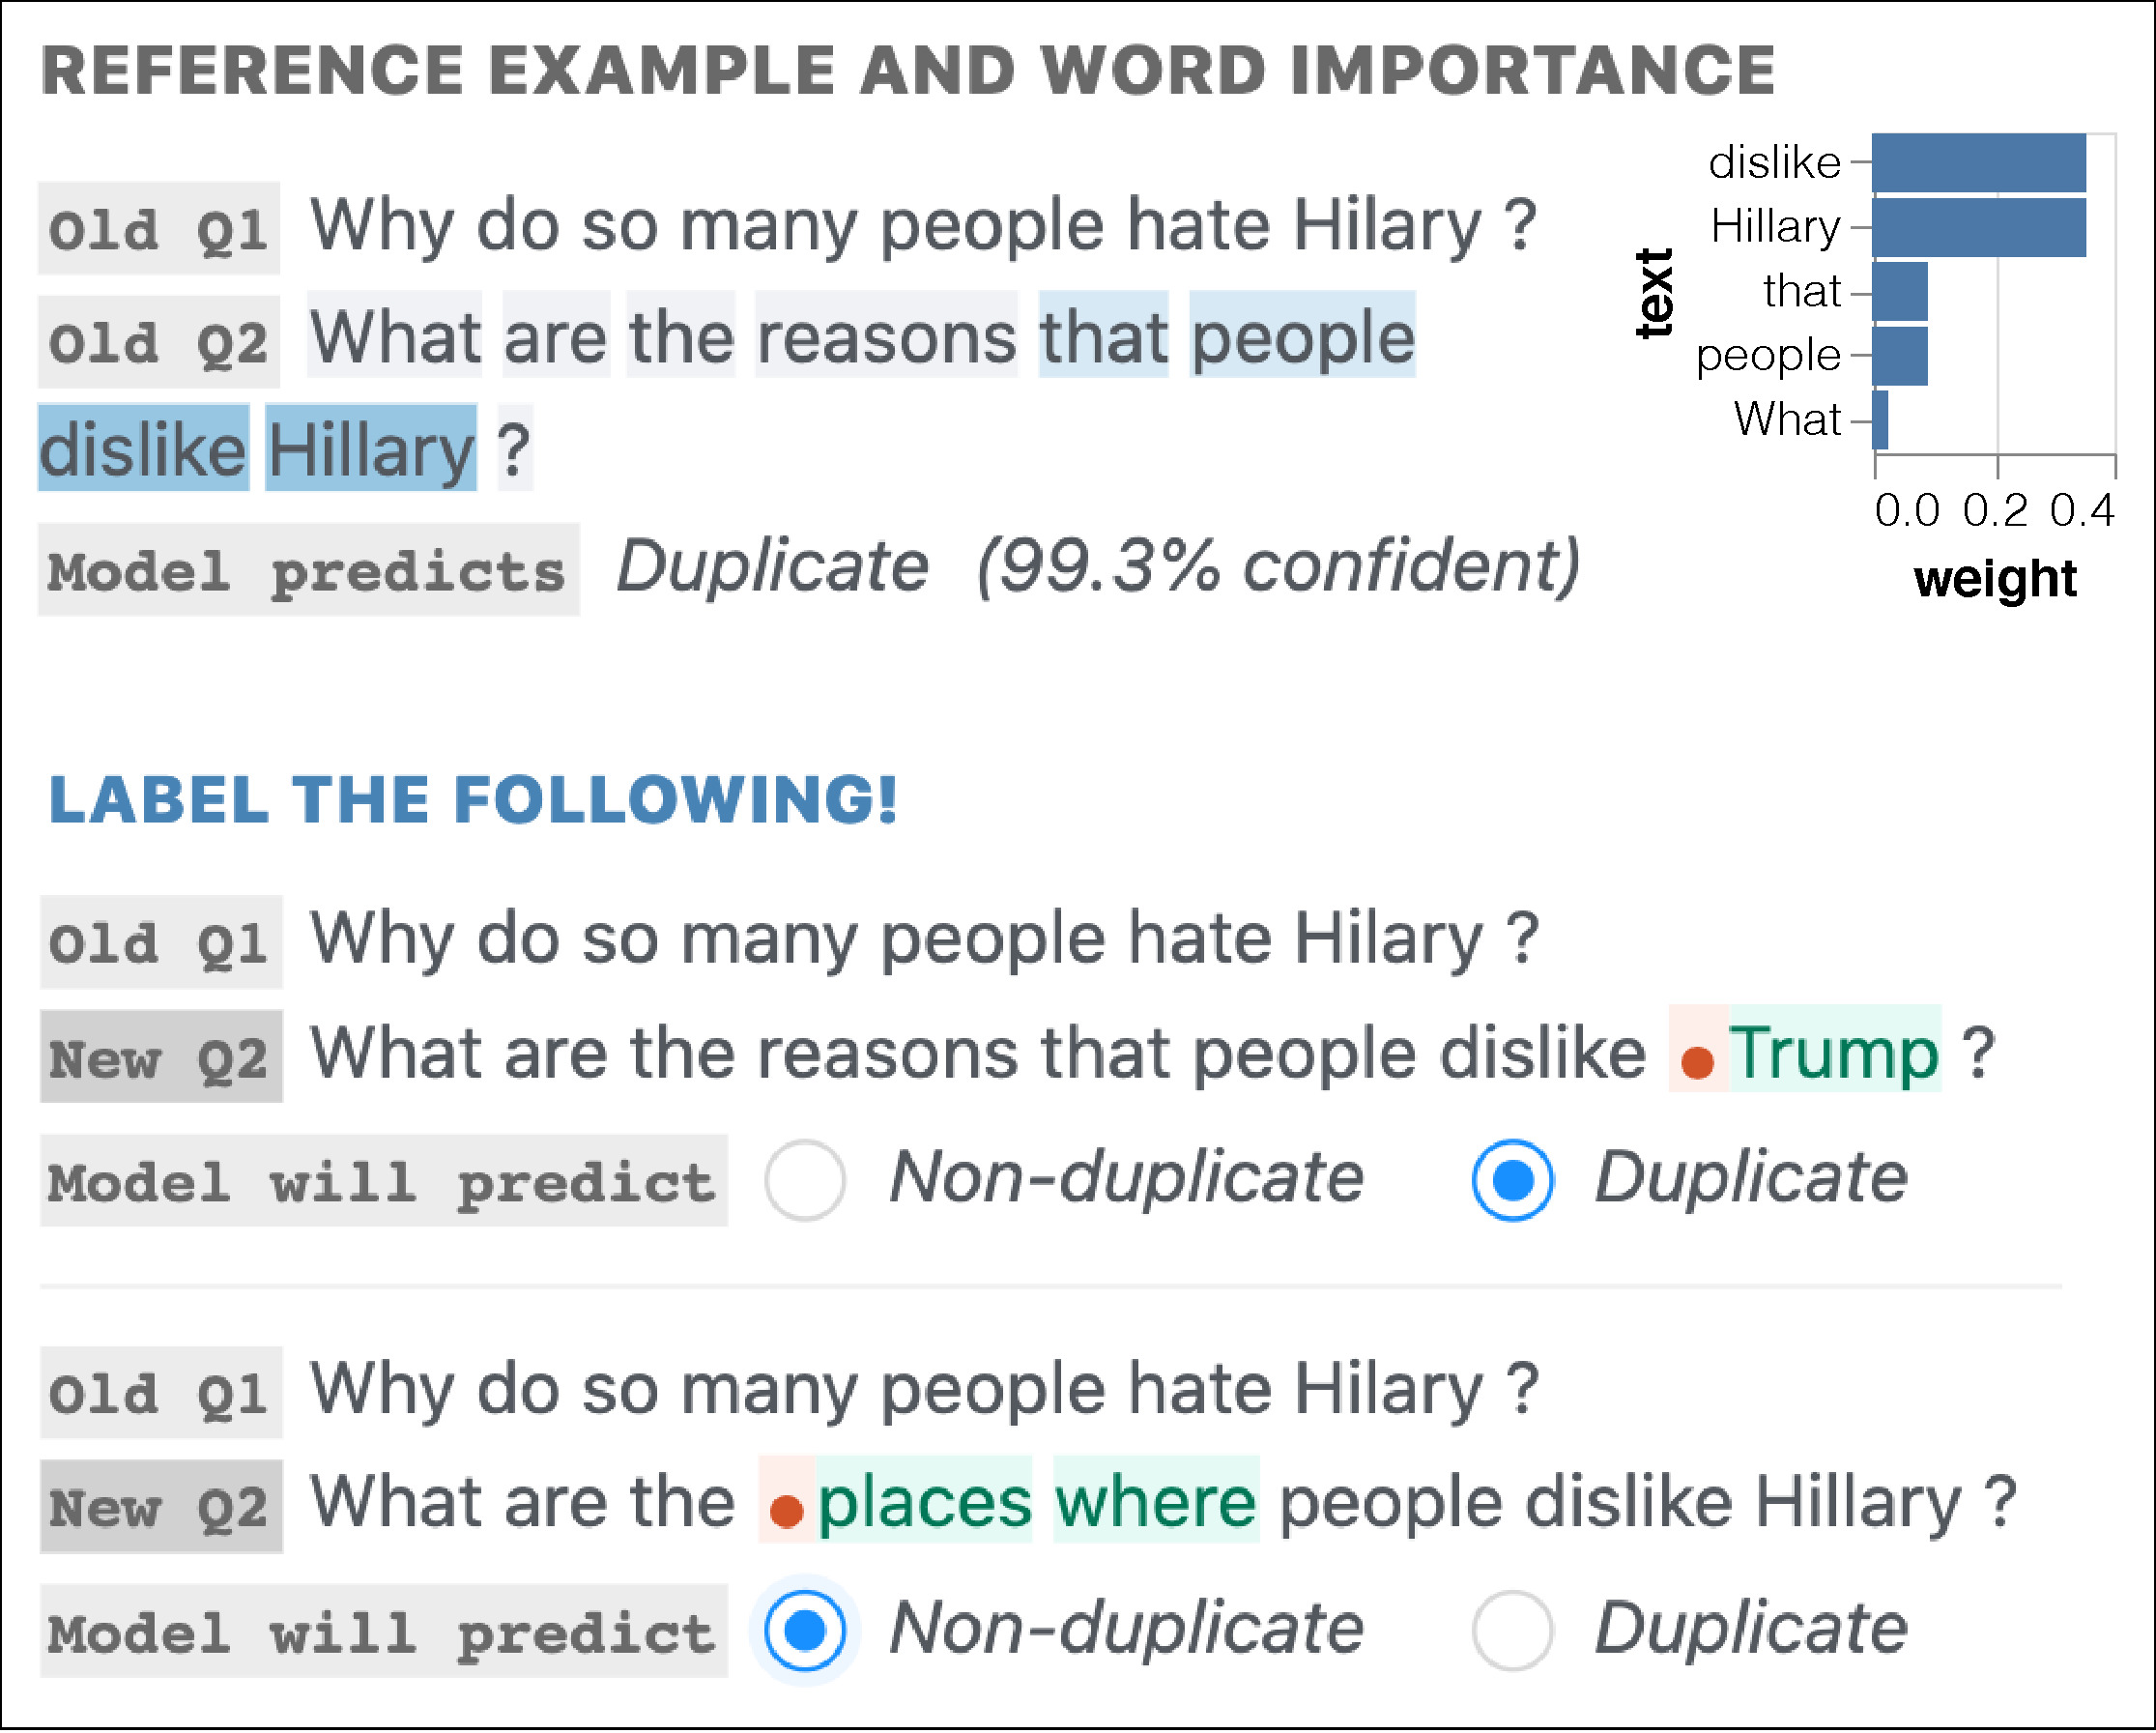
\includegraphics[width=1\columnwidth]{figures/explanation}
\vspace{-15pt}
\caption{}
\vspace{-10pt}
\label{fig:sst_trend}
\end{figure}



\wts{Finding bugs missed by the feature attribution, and concretizing the opaque weights using readable examples.}

\paragraph{Selection by abnormality.}
The cognitive burden of complete explanations is too great.
As a result, \citet{miller} concluded that people usually \emph{select} a small subset of (counterfactual) explanations on contrastive cases (``foils'') that they find unexpected. 
As such, he further proposed that ``abnormality could be used to infer likely foils.''
Here, we operationalize the concept of abnormality based on \emph{the discrepancy between the expected and the actual changes in the prediction}, and use it as our selection method.

Given a prediction model $f$, we define the actual change in prediction as $d_f(\xp, x)$, and the expected prediction change as $\hat{d}_f(\xp, x)$.
The distance between the expectation and reality then becomes:
$$\Delta d_f(\xp, x) = |\hat{d}_f(\xp, x)-d_f(\xp, x)|$$
We select two abnormal, ``turning point'' counterfactuals, \ie unexpected large changes in prediction when small (large) change is expected:
$$ \xp_l = \argmax_{\xp} \Delta d_f(\xp, x), \xp_s = \argmin_{\xp} \Delta d_f(\xp, x)$$
Whereas actual prediction change is always $d_f(\xp, x)=|f(\xp)-f(x)|$ where $f(x)$ denotes the prediction probability of $f$ on $x$, $d_f(\xp, x)$ can take various forms. 
For example, as a standalone explanation method, $\hat{d}_f$ can be the cosine distance in the \emph{Embedding space}.
The embedding can be either model-agnostic (\eg with~sentence transformers~\cite{reimers-2019-sentence-bert}), or the last layer of the hidden state of the finetuned predictor.

On the other hand, as a \emph{compensation} to existing feature attribution methods, $\hat{d}_f$ can be the importance (weights) of the perturbed tokens in $x$, estimated by feature attribution methods.
As mentioned in \wts{\S\ref{}}, methods like SHAP~\cite{} or LIME~\cite{} only estimate feature weights by \emph{masking} the words, which do not represent how model would react in non-deletion counterfactuals (replacing words or inserting negations).
Therefore, abnormalities selected in this way can  compensate or criticize the missed information, and therefore better calibrate users' trust on the predictor.
We primarily test the compensation selection below, as it nicely combines the overview provided by SHAP/LIME, and the decision boundaries omitted by the feature attribution. 
\wts{Add the detail to appendix?}



%%%%%%%
\subsection{Evaluate local explanations?}
We conduct a user study to verify whether our selected counterfactual explanations can compensate SHAP in helping people interpret the model, \ie if the selected counterfactual spot points that people would mis-interpret after viewing SHAP.
We form it as a model behavior simulation study, where participants are asked to predict model's behavior on the given counterfactuals.
Intuitively, the more counterfactuals they simulate incorrectly, the more information they grasp if we show the counterfactuals to them.

\paragraph{Procedure.}
We recruited \wts{N} graduate students who have experience using model explanations before, and asked them to simulate the behavior of a \qqp model for 20 rounds (the same as in \S\ref{subsec:contrast_set}).
In each round, the participants were given a reference example, with the model's prediction on it, its confidence score, as well as the feature attributions estimated by SHAP (\wts{Figure~\ref{}}).
To help them better understand the model around the reference example, the participants were allowed to ``query the model'' for up to 10 times, by making small changes to one question, and see the resulting model predictions.
It was equivalent to unlimited model access --- In the result, most participants submitted \wts{M} queries.
They were then asked to simulate the model's prediction on six counterfactuals, two from each condition.
After the 20 rounds, we concluded the study with open-ended questions on their model query and simulation strategies.

\paragraph{Conditions.} 
We compare three types of selected counterfactuals:
(1) \emph{SHAP-c}, the machine-generated counterfactuals selected to compensate SHAP; 
(2) \emph{random}, the randomly selected machine-generated counterfactuals; 
(3) \emph{human}, 
the human generated counterfactuals that they deemed abnormal.
We allowed three graduate students to play with the model for up to 10 times, and asked them to submit one final counterfactual with a surprising model prediction.
We then randomly selected two of their submissions per reference example.
As a within-subject study, we compared the error rate of human simulations across the three conditions.


\paragraph{Results.}
More interactions with the model usually results in better mental models about the predictor, and users wold become less surprised by most counterfactuals~\cite{miller}.
We are interested in learning whether our selected ones \emph{still add information}
Less surprised by abnormal phenomena, so an explanation alongside every decision runs the risk of providing explanations that become less needed and more distracting over time.

\begin{comment}
****
The examples generated by BERT.
****

  P: The quarterback of the UTEP football team is about to be tackled by a member of the Wisconsin defensive team.
  H: The quarterback is about to be tackled by the opposing team.
 Pr: entailment
 NP: Another quarterback is about to be tackled by the opposing team.
NPr: neutral
weight:  0.122
flip_unimportant_feature 0.013 {The}

  P: The quarterback of the UTEP football team is about to be tackled by a member of the Wisconsin defensive team.
  H: The quarterback is about to be tackled by the opposing team.
 Pr: entailment
 NP: Jack is about to be tackled by the opposing team.
NPr: neutral
weight:  0.461
flip_unimportant_feature 0.028 {The, quarterback}


  P: The quarterback of the UTEP football team is about to be tackled by a member of the Wisconsin defensive team.
  H: The quarterback is about to be tackled by the opposing team.
 Pr: entailment
 NP: The quarterback is about to be tackled by someone
NPr: entailment
weight:  0.218
unflip_important_feature 0.3 {team, the, ., opposing}

  P: The quarterback of the UTEP football team is about to be tackled by a member of the Wisconsin defensive team.
  H: The quarterback is about to be tackled by the opposing team.
 Pr: entailment
 NP: The quarterback is about to be tackled by the second team.
NPr: entailment
weight:  0.292
unflip_important_feature 0.149 {opposing}


\end{comment}


\subsection{Global / Interactive Explanations}
\label{subsec:global_exp}
Here, we explore more extensive use of perturbation explanations via examples, but defer more sophisticated designs and evalautions to future work.

\paragraph{Global explanations: impacts of same changes.}
Going beyond turning points for each individual data points, we can find perturbation patterns that systematically affect (preserve) model predictions.
Similar to challenge sets, the grouped perturbations then become useful for revealing model's capabilities on specific linguistic patterns.

To enable the grouping, we first featurize each perturbation $\xp$ with respect to its original instance $x$, using 
(1) its \tagstr (\fexptag{negation} for the example in Figure~\ref{fig:blank}), 
(2) its remove phrases \fexpfrom{kids}, 
(3) its added phrases \fexpto{not}, \fexpto{children}, and 
(4) the combined template \fexptemp{\swap{kids}{children}}.
For tokens involving multiple changes, we featurize both the primary and the combined changes, and so the example in Figure~\ref{fig:blank} also have additional features like \texttt{\fexptag{negation} \& \fexptag{lexical}}.

For each feature $h$ we compute the its prediction change rate over all the perturbations $\xp \in \xset_{h}$ that have the said feature: 
$R_h = \sum {\mathbb{1}[f(x) \not\eq f(\xp)]} / |\xset_h|$.

Filters on the change rate then reveal different model prediction patterns.\footnote{Because different \nli labels follow very flip patterns, we only include $f(x)=entailment$ examples here}

\noindent\textbf{Mastered patterns.}
Patterns with very high or low change rates (\eg $|R_h-0.5| > \gamma=0.3$) reveal patterns that the model has firmly learned.
In \nli, it includes \fexptemp{\swap{men}{women}} ($R_h=97\%$), \fexptemp{\swap{outdoor}{outside}} ($R_h=0\%$).

\noindent\textbf{Outliers.}
Inspecting the abnormal cases in \emph{mastered patterns}, we find harder to notice examples.
\fexptemp{\swap{three}{four}} changes the 80\% prediction(on 56 changed examples), but all the cases with affected predictions have the explicit pattern ``three'' in the premise, whereas the prediction intact ones show that the model has a hard time processing the actual counting.

\ebox{
\textbf{P}: Three girls fell on top of one another and are laughing.\\
\textbf{H}: \swap{Three}{Four} girls falling and laughing.\\
\textbf{Pr}: \swap{entailment}{contradiction}\\

\textbf{P}: Two little girls and one little boy are running.\\
\textbf{H}: \swap{Three}{Four} kids are running. \\
\textbf{Pr}: \swap{entailment}{entailment}
}

\noindent\textbf{Missed patterns.}
In contrast of the mastered cases, patterns with mild change rates (\eg $|R_h-0.5| < \gamma=0.2$) reveal patterns that the model handles unstably.
For example, the model does not handle the shuffled phrases, echoing the results from \citet{mccoy2019right}.

\ebox{
\fexptag{shuffle}, $R=0.63$ (164 cases)\\
\textbf{P}: The bride in the white dress is surrounded by the groomsmen and bridesmaids, all in black.\\
\textbf{H}: \add{white} woman \remove{in white} is surrounded by others.\\
\textbf{Pr}: \swap{entailment}{entailment}\\

%\textbf{Premise}: Man juggling apples while sitting on a couch with another man on one side and a woman on the other.\\
%\textbf{Hypothesis}: Two \swap{men}{women} sitting near a \swap{woman}{man}.
%\textbf{Prediction}: \swap{entailment}{entailment}\\

\textbf{P}: A man in a wheelchair is being pushed towards a monk.\\
\textbf{H}: The \swap{person is disabled and}{holy person} is being moved towards a \swap{holy}{disabled} person. \\
\textbf{Pr}: \swap{entailment}{entailment}
}


\paragraph{Interactive explanation.}
Besides pre-selected \emph{surprise} cases, perturbations can also support interactive explanation (ideally in a visual interface), and multi-step drill downs.
In the example: 

\ebox{
\textbf{P}: Some dogs are running on a deserted beach.\\
\textbf{H}: There is only one dog at the beach.\\
\textbf{Pr}: contradiction
}

To understand whether the model responses to quantifiers, an analyst can \BLANK ``only one'', which would reveal that the model predicts entailment correct for both perturbed hypotheses:

\ebox{
\textbf{H}: There \swap{is only one dog}{are multiple dogs} at the beach.\\
\textbf{H}: There is \swap{only}{more than} one dog at the beach.
}

Then, the analyst can keep ``more than one dog'' to inspect how the model react to other changes. 
With the model maintaining entailment on the following examples, the analyst would conclude that there may be a strong correlation between NNS and ``more than one,'' that it overwrites many of the prep constraints.

\ebox{
\textbf{H}: There is \emph{more than} one dog at the beach \add{lying down}.\\
\textbf{H}: There is \emph{more than} one dog at the beach \add{inside a cup}.\\
\textbf{H}: There is \emph{more than} one dog at the beach \add{standing}.
}

